\documentclass{INTERSPEECH2023}
\interspeechcameraready 

\usepackage{amsfonts}
\usepackage{url}
\usepackage{multicol}
\usepackage{multirow}
\usepackage{hyperref}
\usepackage{cleveref}
\usepackage[font=small,skip=0pt]{caption}
\usepackage{subfig}
\usepackage{xcolor} % textcolor
\usepackage{cite}
\usepackage{footmisc}

\newcommand{\needcite}{\textcolor{red}{[cite]}}
\newcommand{\fix}[1]{\textcolor{red}{#1}}

\title{Speech Intelligibility Assessment of Dysarthric Speech \\ by using Goodness of Pronunciation with Uncertainty Quantification}
% \title{An improved Goodness of Pronunciation for Automatic Speech Intelligibility Assessment of Dysarthric speech by using Uncertainty Quantification}
\name{Eun Jung Yeo*$^1$\thanks{* Equal contribution.}, Kwanghee Choi*$^2$, Sunhee Kim$^1$, Minhwa Chung$^1$}
%The maximum number of authors in the author list is 20. If the number of contributing authors is more than this, they should be listed in a footnote or the acknowledgement section.
\address{
  $^1$Seoul National University, Republic of Korea\\
  $^2$Carnegie Mellon University, United States of America}
\email{ej.yeo@snu.ac.kr, kwanghec@andrew.cmu.edu, sunhkim@snu.ac.kr, mchung@snu.ac.kr}

\begin{document}

\maketitle

\begin{abstract}
This paper proposes an improved Goodness of Pronunciation (GoP) that utilizes Uncertainty Quantification (UQ) for automatic speech intelligibility assessment for dysarthric speech. Current GoP methods rely heavily on neural network-driven overconfident predictions, which is unsuitable for assessing dysarthric speech due to its significant acoustic differences from healthy speech. To alleviate the problem, UQ techniques were used on GoP by 1) normalizing the phoneme prediction (entropy, margin, maxlogit, logit-margin) and 2) modifying the scoring function (scaling, prior normalization). As a result, prior-normalized maxlogit GoP achieves the best performance, with a relative increase of 5.66\%, 3.91\%, and 23.65\% compared to the baseline GoP for English, Korean, and Tamil, respectively. Furthermore, phoneme analysis is conducted to identify which phoneme scores significantly correlate with intelligibility scores in each language.
\end{abstract}
\noindent\textbf{Index Terms}: dysarthric speech, speech intelligibility, automatic assessment, goodness of pronunciation, uncertainty quantification

% with the best-performing GoP  

% The current GoP method relies heavily on acoustic model predictions, which have limitations of network-driven overconfident predictions. 


%The experiment used phoneme probabilities from a fine-tuned Wav2Vec XLS-R model. GoP with prior-normalized maxLogit showed the best performance, with a relative increase of 5.66%, 3.91%, and 23.65% compared to the baseline for English, Korean, and Tamil, respectively. Additionally, the proposed GoP was used to conduct phoneme analysis to identify which phoneme scores significantly correlate with intelligibility scores in each language.









% Using Kendall's rank coefficient between GoP and intelligibility scores, we aim to find the optimal UQ method for dysarthria assessment.
% 998/1000

% Although GoP has shown successful performances in language education applications, applications on disordered speech has been limited.


% The model's probabilities are then used to calculate GoP.

% For further improvements, each measurement is normalized by incorporating UQ methods into the phoneme recognizer.

% The proposed method is tested on English, Korean, and Tamil dysarthric speech datasets, and all measurements except entropy perform better than the baseline, GMM-GoP and NN-GoP. The best-performing measurement improves by an average of 31.98% and 2.63% relative to GMM-GoP and NN-GoP, respectively. Additionally, the paper analyzes which phonemes significantly correlate with intelligibility scores for each language.


% We explore seven new GoP measures by modifying 1) the scoring function and 2) the phoneme predictor. 

% 978/1000 characters. ASCII characters only. No citations.
% No italics, non-ASCII characters

% Further analysis is conducted to find the frequently mispronounced phones by severity levels and languages.

% However, recent studies claim that predictions from neural networks are often over-confident.

% However, previous studies have limitations in giving over-confident results and being heavily dependent on language-dependent acoustic models.

% However, predictions of modern neural networks have the limitations of giving over-confident results.

% Further analysis is conducted to find the frequently mispronounced phones by severity levels and languages.

% This phenomenon can hinder the performance of GoP, which heavily depends on the phone probability of language-dependent phone recognition models.


% Kendall's rank coefficient between the expected pronunciation scores and the intelligibility severity levels is compared to the traditional methods.

% Previous studies have proposed variations of Goodness of Pronunciation (GoP) to score the similarity of pronounced phones with canonical phones.

% this paper presents an attempt to utilize Goodness of Pronunciation (GoP) with uncertainty quantification for phone-level pronunciation scoring and assessment of dysarthric speech.
% Degraded speech intelligibility due to misarticulated phones is one major characteristic of dysarthric speech.

% We utilize representations extracted from the convolutional layer of the Wav2Vec2.0 XLS-R model, which have been revealed to contain abundant acoustic features.

% However, the methods have two limitations: (1) dependency on acoustic models, and (2) uncalibrated results of the neural networks.

% The common way of phone-level scoring and assessment is conducted with GoP.

% The XXX method presents the best performance, achieving the coefficient of XX.

% While phone-level pronunciation scoring has often been applied to non-native speech, applications to atypical speech have been limited.

% We further conduct analysis on the frequently mispronounced phones by severity levels and languages.


% due to its nature of high dependence on phone probaiblity from acoustic models.  
% As the traditional way of automatic pronunciation scoring measure, variations of GoP have been proposed to assess atypical speech, by leveraging modern neural networks (NN).
% However, recent studies have reported that NNs produce overly confident predictions, which can 
% , which heavily relies on phone probability from acoustic models. 

% Previous studies have leveraged neural networks in proposing variations of GoP.
% However, studies have reported that modern neural netowkrs have the tendency to produce overly confident predictions, which 

% However, modern neural networks are known to produce overly confident predictions. 
% This negatively impacts traditional GoP performance, which heavily relies on phone probability from acoustic models. 
% With UQ methods having shown to alleviate overconfidence of the neural networks,

% GoP is the traditional way of assessing pronunciations of atypical speech.
% While variations of GoP have been suggested by leveraging the development of neural networks (NN), recent research reported that NNs produce overly confident predictions. 
% This negatively impacts GoP performance, as the measures heavily rely on phone probability from acoustic models. 
% To alleviate the problem, this paper proposes to incorporat UQ methods into GoP.

% As dysarthric speech exhibits great intra-speaker and inter-speaker variability, modifications to normalize the probabilities are necessary for optimal GoP performance. 
% Phone probabilities are extracted from a cross-lingual XLS-R model fine-tuned with healthy speech.
% Then, UQ methods are applied to normalize the acoustic deviations of each phonemes in two ways.
% First, probabilities are replaced with new phoneme predictions.
% Second, such predictions are normalized with each phoneme probability. 
\section{Introduction} \label{sec:intro}
% P1 What is dysarthria? % Why is intelligilbity assessment important? 
Dysarthria is a motor speech disorder caused by weakness or paralysis of the articulators \cite{darley1972dysarthria}.
People with dysarthria often suffer from degraded speech intelligibility, repeated communication failures, and ultimately low quality of life. 
Accordingly, dysarthric speech assessments regarding speech intelligibility are conducted to check the patient's status and track the effectiveness of treatments \cite{kent1989toward}.
While the common way of dysarthric speech assessment is perceptual evaluation, the method is often subjective and laborious. 
Therefore, automatic speech assessment with objective and rapid results can assist clinicians in diagnosis and treatment planning.

%auxiliary diagnosis of clinical medicine

% To overcome such issues, research on the automatic assessment of dysarthric speech has been proposed, to assist clinicians' diagnoses and treatment planning with objective, reliable results.

% Hence, the automatic classification that highly correlates with the experts will have great potential for aiding clinicians in diagnosis and speech therapy.

% P2: Previous research 1
% Raw feature : Low Interpretability 
% Hand-crafted feature: Feature may be lossy
There are two main approaches to automatic assessment
of dysarthric speech. 
The first approach is to propose a list of hand-crafted features that are expected to capture the characteristics of dysarthric speech.
Explored feature sets include voice quality features \cite{narendra2021automatic}, prosody features \cite{hernandez2020prosody}, articulation or pronunciation features \cite{kim2012automatic, liu2021language}, and their combinations \cite{vasquez2018towards, yeo2022multilingual}.
This approach has the benefit of having medical implications, as it provides a transparent understanding of the features employed for automatic assessment. 
Nevertheless, this approach has the drawback that features that could be valuable in the assessment could be discarded during feature extraction.
The second approach involves leveraging the capabilities of neural networks (NNs), which can achieve better results by using raw inputs. \cite{yeo2022automatic, joshy2023dysarthria}.
% This method achieves better performance than the former method, with the benefit of allowing the model to self-learn the important features for the task. 
However, due to the black-box nature of NNs, the approach limits interpretability, which clinicians often crave for.

% karjigi2023speech
% P3: Previous 2
% Interpretable Neural Networks
 % Interpretability is important for clinical usage --> previous studies: CNN (sondes) 
\begin{figure}[t] %%% t: top, b: bottom, h: here
\centering
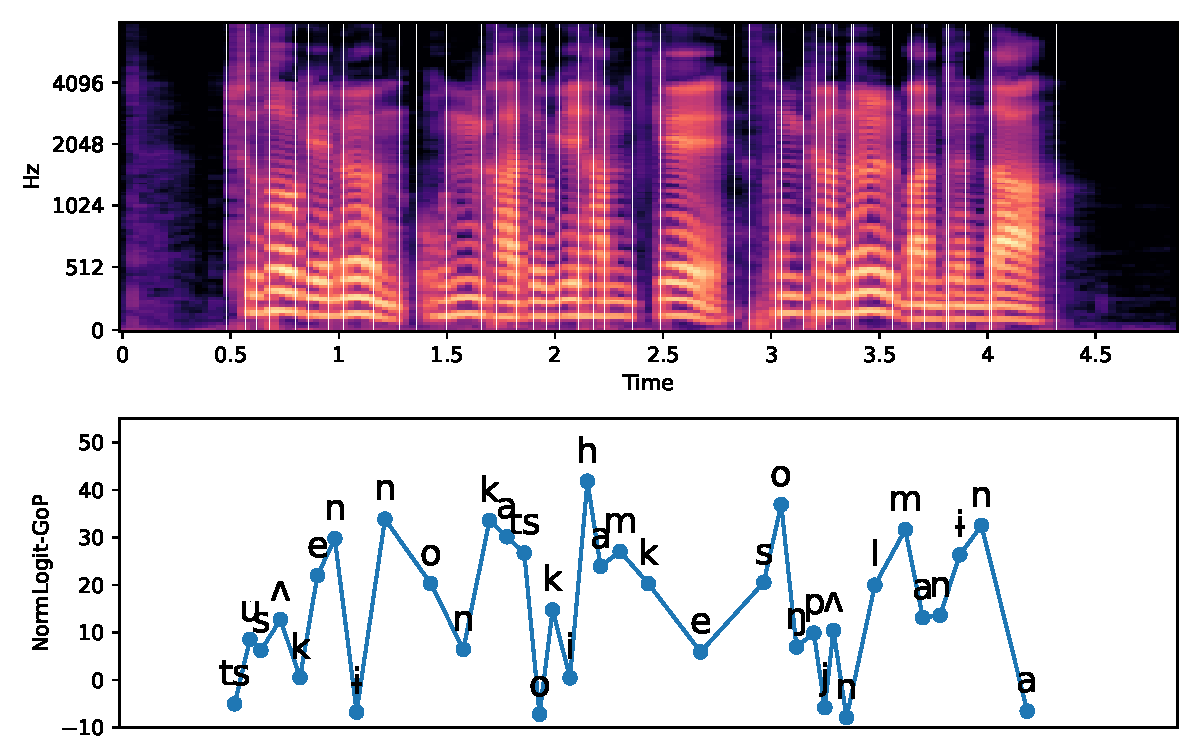
\includegraphics[width=0.97\columnwidth]{figures/fig_samplewise_gop.pdf}
\caption{
Example of GoP scores for each phone within an utterance.
Higher values indicate greater deviation from the correct pronunciation.
GoP scores allow easy identification of mispronounced phonemes.
}
\vspace{-1em}
\label{figs:samplewise_phones}
\end{figure}
Recent studies have attempted to integrate the benefits of both approaches, by enforcing the neural networks to learn the intermediate labels used for perceptual assessment, such as voice quality, articulation precision, nasality, and prosody \cite{tu2017interpretable, xu2021explore}.
Furthermore, certain studies focused on decoding misarticulation characteristics, which are the prominent aspect of dysarthric speech across languages \cite{yeo2022multilingual} and a significant factor that influences speech intelligibility \cite{de2002intelligibility}. 
For instance, the framework that measures the level of phonetic impairment was proposed by utilizing the activations of the hidden neuron \cite{abderrazek2022interpreting, abderrazek2022validation}.
While the method could provide overall phonetic characteristics of utterances, it is unable to provide assessments at the level of individual phonemes, which can help clinicians to pinpoint specific phonemes that require pronunciation training.

% which is essential for clinical applications such as pronunciation training.

% However, although the approach could offer information on averaged phonetic features of utterances, it did not provide phoneme-wise evaluations that are necessary to pinpoint specific phonemes that require improvement in clinical applications, such as pronunciation training. 

A common approach of phoneme-level speech assessment is to use the parallel NN that employs parallel datasets. 
The NN was trained using the same set of utterances recorded by both healthy speakers and patients to learn how to distinguish whether each phone in the utterances was from healthy or disordered speech \cite{miller2020assessing,quintas2022automatic}.
However, obtaining parallel datasets is a challenging task, especially for disordered speech.
Moreover, this approach often constrains the analysis to pre-defined speech materials, which may not capture the natural speech patterns utilized in everyday communication.

% For example, previous studies have utilized diadochokinetic exercises or pseudo-words as speech materials, which may not be representative of natural speech patterns.
% Furthermore, this limits the analysis to specific types of speech materials, which may not be representative of natural speech used in everyday communication, such as diadochokinetic exercises in \cite{miller2020assessing} and pseudo-words in \cite{quintas2022automatic}.


% P4: Misarticulation is the one of the major charactersitcs of dysarthria: Interpretability 를 개선하기 위해 GOP를 improve
% GOP + disordered speech
% GOP + wav2vec
\begin{figure*}[t!] % t: top, b: bottom, h: here
\centering
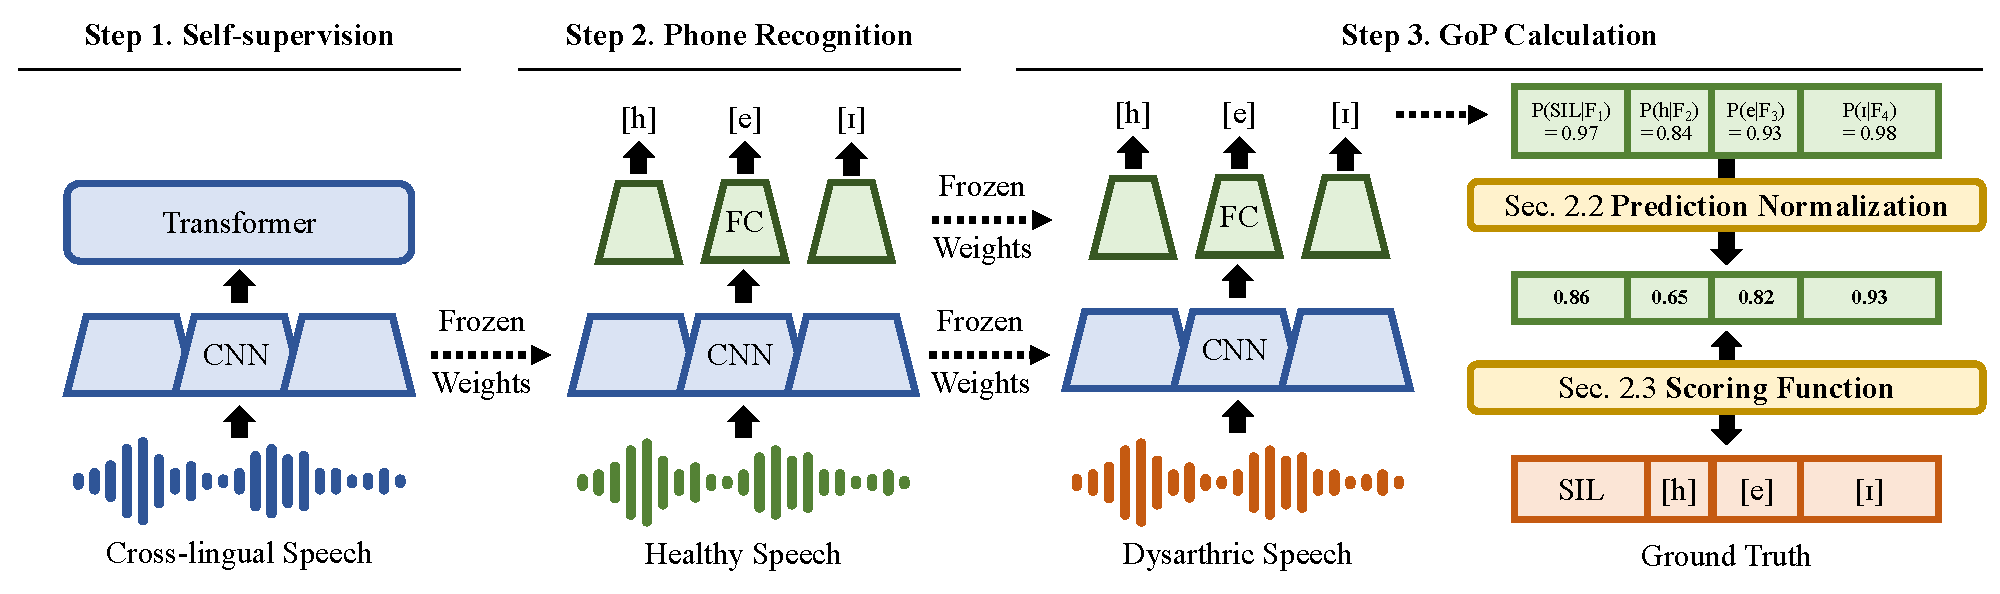
\includegraphics[width=1\textwidth,height=5cm]{figures/dysarthria-gop.pdf}
\caption{Overview of the improved GoP with UQ methods.}
\vspace{-1em}
\label{fig:diagram}
\end{figure*}

Another conventional approach of phoneme-level pronunciation evaluation is Goodness of Pronunciation (GoP) \cite{witt2000phone}.
GoP, which is defined as the degree of similarity between produced and correct pronunciation of phonemes, has two advantages in automatic speech assessments.
First, it provides detailed information on which phonemes are mispronounced and to what extent each phoneme is atypical.
Second, it does not necessitate a parallel dataset for model training.
% the approach eliminates the need for parallel recordings of healthy and atypical speech, making it a valuable tool for practical applications.
While GoP is often applied to non-native (L2) speech pronunciation assessment, some studies have also verified its potential use in assessing speech disorders as well \cite{pellegrini2014goodness,Fontan2015PredictingDS}.
% For example, the GoP-based assessment model correctly detected mispronounced phonemes from French-speaking unilateral facial palsy patients \cite{pellegrini2014goodness}. 
% Additionally, GoP showed strong correlations with comprehensibility ratings for diverse types of French-speaking patients \cite{Fontan2015PredictingDS}.


% Thus, to ensure optimal performance, it is crucial to consider the standardization of phone probabilities for GoP, as it relies heavily on acoustic model probabilities.
With the development of NNs, variants of GoP which employ probabilities from the state-of-the-art neural networks have been suggested \cite{hu2015improved,Cheng2020ASRFreePA,xu2021explore}.
However, using these probabilities without taking into account the modern NNs' tendency towards overconfidence can result in inaccurate conclusions:
NNs often generate probabilities close to $1.0$ even when their predictions are incorrect \cite{guo2017calibration}.
Since GoP relies heavily on probabilities, this can be especially problematic. The issue is compounded when the model encounters out-of-distribution (OOD) inputs, which are data that differ significantly from the training data's distribution \cite{hendrycks2017baseline}, such as dysarthric speech for healthy speech.
To alleviate such issues, UQ techniques, techniques to combat OOD problem \cite{guo2017calibration,hendrycks2017baseline}, can be applied.

% However, naive use of the probabilities from NN may lead to misleading conclusions due to the inherent overconfidence of modern NN.
% That is, NNs are often reported to output probabilities close to 1 even when their predictions are incorrect \cite{guo2017calibration}. 
% While this behavior can be critical to GoP as it heavily relies on probabilities, it becomes more problematic when the model encounters out-of-distribution (OOD) inputs, which refers to data that significantly differs from the distribution of the training data \cite{lee2018simple}. 
% To alleviate the issues, attempts to quantify uncertainty have been proposed, which is known as Uncertainty Quantification (UQ) methods. 

% Since GoP relies heavily on probabilities, this can be especially problematic. The issue is compounded when the model encounters out-of-distribution (OOD) inputs, which are data that differ significantly from the training data's distribution. To address these issues, researchers have proposed methods to quantify uncertainty, known as Uncertainty Quantification (UQ) methods.



% Dysarthric speech, like pathological speech, can be classified as OOD input since it differs greatly in acoustics from healthy speech. This paper proposes enhanced GoP variants for dysarthric speech evaluations by utilizing conventional Uncertain Quantification (UQ) techniques, which are known to tackle the OOD problem.

% directly applying methods from L2 assessment can result in suboptimal results. 
% In fact, a study on the analysis of L2 and disorder speech have shown different aspect \cite{}
% This issue becomes more problematic when the model encounters out-of-distribution (OOD) inputs, such as pathological speech that the model has not encountered during training \cite{lee2018simple}. 

This paper proposes improved GoP for automatic speech intelligibility assessment for dysarthric speech by employing Uncertainty Quantification (UQ) methods in two ways: (1) normalizing the phoneme prediction and (2) modifying the scoring function.
As pathological speech greatly differs in acoustics from healthy speech \cite{wilson2000acoustic}, dysarthric speech can be also understood as OOD input.
Therefore, we employ conventional UQ methods to improve GoP calculations for dysarthric speech assessment.
To assess the effectiveness of the improved GoP with UQ techniques, three dysarthric datasets, namely, UASpeech English, QoLT Korean, and SSNCE Tamil dataset, are utilized. 
To summarize, this paper redefines the current versions of GoP from a UQ standpoint and evaluates the effectiveness of UQ methods in improving GoPs.


% This paper aims to improve GoP for automatic speech intelligibility assessment of dysarthric speech, by regarding dysarthric speech as OOD samples for the NN.
% Hence, the Uncertainty Quantification (UQ) methods, which is a conventional technique to combat OOD problems, is applied on phoneme probabilities extracted from the fine-tuned Wav2Vec XLS-R model. 
% To check the efficacy of our improved GoP with UQ method, we use three dysarthric datasets, which include TORGO English, QoLT Korean, and SSNCE Tamil dataset.
% To sum up, this paper redefines the existing variants of GoP through the lens of UQ perspective, and verifies the efficacy of the conventional UQ methods for improved GoP.


% This paper presents improved GoP variants for automatic speech intelligibility assessment of dysarthric speech, by using Uncertainty Quantification (UQ) methods.
% UQ is a set of techniques used to estimate and understand uncertainty, and has been reported to show great performances in various domains.
% However, naive use of the NN may lead to misleading conclusions due to the inherent overconfidence of modern NN \cite{guo2017calibration}.
% That is, modern NNs often output probabilities close to 1, even when the network's predictions are incorrect.
% This issue becomes particularly problematic when the NN is presented with out-of-distribution (OOD) inputs, such as pathological speech, which the model has not seen during training \cite{lee2018simple}. 
% In fact, the vast acoustic difference of dysarthric speech from healthy speech have often impeded the technology applications developed for healthy speakers \cite{wilson2000acoustic}.

% Therefore, this paper considers pathological speech OOD input.


% This becomes especially problematic when NN has never seen the sample during training, often defined as out-of-distribution (OOD) inputs \cite{lee2018simple}.
% Considering its vast acoustic difference from healthy speech, pathological speech may be considered as OOD input. 
% Moreover, some studies reported \cite{}.
% Hence, directly applying methods from L2 assessment can result in suboptimal results \cite{wilson2000acoustic}.







% is known to help the model to combat miscalibration techniques. \cite{guo2017calibration,hendrycks2017baseline}.
% Therefore, 
% We revisit the existing variants of GoP through the lens of UQ and apply simple yet effective methods to improve upon them.



% However, predictions of modern neural networks have the tendency to produce uncalibrated and overconfident predictions \cite{guo2017calibration}.
% However, earlier investigations on GoP have neglected the significant intra-speaker and inter-speaker variability present in dysarthric speech. which can impede the application of other technologies on this type of speech \cite{wilson2000acoustic}. 



% , as it offers phoneme-level information without requiring parallel datasets.

% to combat its miscalibration.



% The rest of the paper is organized as follows: \Cref{sec:gop} introduces the improved GoPs by using the UQ methods. 
% \Cref{sec:experiment} describes the experiments, including datasets and details of our implementations for both baseline and proposed experiments.
% Results regarding the performances of the experiments and further analyses of essential phonemes for speech intelligiblity by languages are demonstrated in \Cref{sec:results}.
% Lastly, \Cref{sec:conclusion} is followed with a conclusion.

% by utilizing neural networks as a component inside the existing theoretical framework. 
% Some studies have sought to explain the neural network's decisions in terms of multiple dimensions such as vocal quality, articulation precision, nasality, and prosody \cite{tu2017interpretable, xu2023dysarthria}.
% While the approach can provide a comprehensive view of speech features, they cannot provide in-depth information for each aspect, which may have practical applications for clinical intervention. 

% The fundamental idea of applying GoP to disordered speech is to detect pathological phonemes that are different from that of healthy speech.

% Mispronounced phonemes can be identified using a threshold, which is often optimized using a validation set \cite{hu2015improved, xu2021explore}. 

% Hence, this paper utilizes GoP for automatic speech intelligibility assessment of dysarthric speech.


%%%again..
% This paper proposes an improved GoP for automatic speech intelligibility assessment of dysarthric speech, by using Uncertainty Quantification (UQ) methods.
% However, there are two drawbacks of existing GoP approaches, regarding the characteristics of dysarthric speech: (1) the scoring function is not expressive enough to capture uncertainty, and (2) the output phoneme prediction probabilities are uncalibrated.
% Hence, Uncertainty Quantification (UQ) methods are incorporated in GoP calculations, by (1) updating the scoring function and (2) modifying the phoneme predictor.
% UQ is a set of techniques used to estimate and understand uncertainty, and is known to help the model be more accurately calibrated, leading to more reliable predictions and better decision-making \cite{guo2017calibration,hendrycks2017baseline}. 
% To standardize the skewed phone probabilities, which is a notable characteristic of dysarthric speech, we anticipate that the inclusion of UQ will be beneficial for GoP calculations.
% To validate the effectiveness of our proposed method, three dysarthric datasets are tested, which includes  English, QoLT for Korean, and SSNCE for Tamil.

% This addresses two main shortcomings of existing GoP approaches, namely the insufficiently expressive scoring function and the uncalibrated phoneme prediction probabilities.
% UQ method is the technique have been proposed to correct bias in various research fields, such as computer vision and natural language processing (NLP) \needcite. 

% Hence, we improve GoPs by using UQ methods, which have been suggested to rectify bias in 

% In addition, to further reduce the language-specificness of the phoneme predictor, we leverage the recently introduced self-supervised model with cross-lingual training \cite{babu22_interspeech} to extract the speech features.


% The rest of the paper is organized as follows: \Cref{sec:gop} introduces the proposed approach of improving GoP by using the UQ methods. 
% \Cref{sec:experiment} describes the experiments, including the experimental setup of our implementations.
% Results regarding the performances of the experiments and further analyses of frequently mispronounced phones by languages are demonstrated in \Cref{sec:results}.
% Lastly, \Cref{sec:conclusion} is followed with a conclusion.


%Kaldi-based; GoP based: need largae amount of data for training


% Previous studies have leveraged the development of neural networks to propose variations of GoPs.
% Started from GMM-GoP \cite{witt2000phone}, studies proposed to calculate GoPs from Time-delayed neural network (NN-GoP) \cite{hu2015improved}, generative model \cite{Cheng2020ASRFreePA}, and Wav2Vec 2.0-based model \cite{xu2021explore}. 
% However, predictions of modern neural networks have the tendency to produce uncalibrated and overconfident predictions \cite{guo2017calibration}.
% That is, even when the network's predictions are incorrect, the model often outputs probabilities close to 1.
% % This greatly degrades the trustworthiness and reliability of neural networks. 
% Considering GoP is highly dependent on the probabilities of the neural networks, such bias can greatly hinder the performance of GoPs. 
% To address these concerns, uncertainty quantification (UQ) techniques have been suggested to rectify bias in various research fields such as computer vision and natural language processing (NLP) \needcite.
% Therefore, this paper incorporates UQ methods in the speech domain, particularly, in GoP score calculations for dysarthric speech assessments.

% Given the numerous advancements of UQ methods, the natural progression of it is to apply them to GoP.

% especially for tasks such as confidence calibration and out-of-distribution (OOD) detection.
% Confidence calibration aims to match the prediction probabilities to represent the true correctness likelihood \cite{guo2017calibration}, and OOD detection tries to detect the samples that are highly different from the training samples \cite{lee2018simple}.

% P5: Propose model
% Phone-level assessment method of dysarthric speech
% Focus on improving the well-known examination of phone-level assessments: Goodness of Pronunciation (GOP)
% we suggest a novel way of understanding the GOP predictions with the lens of out-of-distribution detection, where numerous advances have been made on OOD in the past decade.
% other ood methods도 활용해서 보여주겠다
% we further leverage the power of cross-lingual self-supervision to avoid the language bias inherent inside the acoustic models of GOP




% and \Cref{sec:discussion} further demonstrates analyses of frequently mispronounced phones by severity levels and languages detected by our best-performing method. Lastly, \Cref{sec:conclusion} is followed with a conclusion.

%performance of proposed models is evaluated with existing mainstream methods

% for classification. \Cref{sec:speech_corpus} presents three datasets: TORGO for English, QoLT database for Korean, and SSNCE database for Tamil. Finally, \Cref{sec:setup} describes the experimental settings and reports classification results, which is followed by a conclusion in \Cref{sec:dis_con}.

% Contribution
%% Detailed Assessment Results with phone-level assessment
% 기존 GOP를 OOD로 재해석해서 성공적으로 잘활용되고 있는 OOD의 literature를 사용.
% Rethinking of 

% ------------

% P5 Propose model
% SSL representations + OOD 사용



% asr-dependency
% prob 1: asr 성능을 높이려면: ctc/rnn-t -> acoustic model만 있는게 아니고, language model 능력도 transformer에다가 밀어넣음. (food: fud -> fo[sep]od -> "food"라는 단어를 이해 -> 앞뒤를 보고 넣은거 -> receptive field가 전체를 보고 있음 vs. phoneme recognition (local하게 phone 제대로 발음했니?)
% -> target: phone (ipa) -> inherently introduces language independence
% prob 2: softmax() -> inherently dependent on other phone class prob. -> [0.5, 0.5] = (1) 둘다 probable하다 (2) 둘다 improbable하다
%   

% One aspect is to explain articulatory or pronunciation characteristics  
% For exmplae, studies have focused on analyzing articulation or pronunciation, which plays a significant role in speech intelligibility \cite{de2002intelligibility}. 

%--------------------------------------------
% consonant-vowel transition, 
% For example, a jointly trained fully-connected neural network with a severity label at the output layer and four perceptual labels (nasality, vocal quality, articulatory precision, prosody) at the intermediate layer was proposed \cite{tu2017interpretable}.
% The model demonstrated better accuracy and interpretability, by explaining the final decisions with a set of explanatory features, which include nasality, vocal quality, articulatory precision, and prosody. 
% Another study trained the CNN-based model to jointly learn a classification label and four clinically-interpretable features, by adding an interpretable layer after the output layer.
% Interpretable layer consisted of four units, each learning the acoustic aspects of articulation precision, consonant-vowel transition precision, hypernasality, and vocal quality \cite{xu2023dysarthria}.
% In addition, Shapley additive explanation (SHAP) was applied to further analyze the contribution of each acoustic feature in the interpretable layer to the final prediction.
% The interpretable layer consisting of 4 units are trained to learn the acoustic features that characterizes different aspects of dysarthria interpretable to clinicians.

%-------------------------------------------
% Previous studies includes Neuro-based Concept Detector \cite{abderrazek2022interpreting, abderrazek2022validation}, 

% On the other hand, some studies focused on the analysis into misarticulation, which is the prominent characteristic of dysarthric speech across languages \cite{yeo2022multilingual}.
% Neuro-based Concept Detector was demonstrated to reflect the level of impairment of the phonetic features through its hidden neurons' activation patterns \cite{abderrazek2022validation,abderrazek2022interpreting}.
% Features using phonological posterior probabilites obtained by parallel bi-directional recurrent neural networks were used to determine the severity level of dysarthria \cite{miller2020assessing}.
% The automatic prediction model based on a siamese network that computes similarity scores between healthy and pathological consonants were proposed \cite{quintas2022automatic}.
% This study also aims to investigate the incorrectly pronounced phonemes and utilize this information for automatic speech intelligibility assessment of dysarthric speech.

 % to promote interpretability in terms of the pronunciation of the consonants 
%comprehensive %auxiliary diagnosis of clinical medcine

% An objective articulation measure of the consonant-vowel transitions was derived based on the posteriors of a convolutional neural network \cite{mathad2022consonant}.



% Some studies have sought to explain the neural network's decisions in terms of multiple dimensions such as vocal quality, articulation precision, nasality, and prosody \cite{tu2017interpretable, xu2023dysarthria}.
% While the approach can provide a comprehensive view of speech features, they cannot provide in-depth information for each aspect, which may have practical applications for clinical intervention. 

% Other studies concentrated on the analysis of phoneme-level pronunciation \cite{miller2020assessing,quintas2022automatic}.
% Although such models may not generate extensive interpretable insights provided by previously-mentioned studies, they have an advantage in offering information on what phonetic features or phonemes are atypical.

% Therefore, this study adopts the second approach, and examines mispronounced phonemes and utilizes the information for automatic speech intelligibility assessment of dysarthric speech.

% a prominent characteristic of dysarthric speech across languages \cite{yeo2022multilingual}, and 

% Another approach is to analyze the activation patterns of the hidden neurons associated with phonetic features 

% With such advantages, GoP has been utilized to automatically assess atypical speech, including non-native speech \cite{} and disordered speech \cite{}.

% Variations of GoP have leveraged the development of neural networks. 
% While GMM-GoP was the starting point \cite{witt2000phone}, subsequent studies proposed calculating GoPs from Time-delayed neural networks (NN-GoP) \cite{hu2015improved}, generative models \cite{Cheng2020ASRFreePA}, and Wav2Vec 2.0-based models \cite{xu2021explore}. 
% However, modern neural networks tend to generate uncalibrated and overly confident predictions. 
% That is, even when they are incorrect, leading to probabilities close to 1 \cite{guo2017calibration}. 
% Since GoP heavily depends on the neural networks' probabilities, such biases can significantly impede the performance of GoPs. 
% To address these concerns, uncertainty quantification (UQ) techniques have been proposed to correct bias in various research fields, such as computer vision and natural language processing (NLP) \needcite. 
% Therefore, this paper introduces UQ methods in the speech domain, particularly in GoP calculations.

% To overcome these issues, this paper employs Goodness of Pronunciation (GoP) for automatic speech intelligibility assessment in dysarthric speech. 
% Goodness of Pronunciation (GoP) is the metric that scores pronunciation of atypical speech at a phoneme level.
% GoP uses the posterior probability of the correct phone, obtained from acoustic models, along with the speech segment of the corresponding phone \cite{witt2000phone}. 

% However, parallel networks often require parallel datasets in training the models to recognize and differentiate between various phonemes or speech sounds due to the difficulty in obtaining parallel datasets. 
% obtaining these parallel datasets can be particularly challenging for disordered speech datasets, which makes it difficult to obtain matched speech samples between individuals with speech disorders and healthy speakers.
% Despite the promising results, parallel networks often require parallel datasets to train the models to recognize and distinguish between different phonemes or speech sounds, which is often difficult to be obtained for disordered speech dataset.
% Without parallel datasets, it can be challenging to train the network to differentiate between the target phonemes and other sounds that may be present in the speech signal.
% , which is challenging for disordered speech corpus. 

% Likewise, parallel networks often require parallel datasets, to train the models to recognize and distinguish between different phonemes or speech sounds.
% This limits the applications in a clinical setting, as it is difficult to obtain parallel datasets.
% One of the major limitations of parallel networks is that they often require parallel datasets to train the models to effectively recognize and differentiate between various phonemes or speech sounds. 

% However, the research was limited to diadochokinetic exercises. 
% Again, the study constrains the materials to 52 pseudo-words.

% However, this study was also limited in that it used only 52 pseudo-words as materials.

% This can pose a challenge in a clinical setting, particularly for disordered speech datasets, as obtaining appropriate parallel datasets can be difficult due to the idiosyncratic speech patterns and individual differences in speech production. Therefore, while parallel networks have shown potential for phoneme-level assessments, the need for parallel datasets can limit their applications in clinical settings.


% For instance, parallel bi-directional recurrent neural networks were presented to extract phonological posterior probabilities to assess the severity level of dysarthria \cite{miller2020assessing}.
% % Another study proposed the use of a siamese network to compute similarity scores between healthy and pathological consonants, in order to predict intelligibility scores for Head and Neck Cancer speech \cite{quintas2022automatic}.
% However, parallel networks often require parallel datasets to train the models to effectively recognize and differentiate between various phonemes or speech sounds.
\section{Proposed approach} \label{sec:gop}
The study applies various conventional UQ methods to calculate GoP scores, which are demonstrated in \Cref{fig:diagram}.
We release the source code of all the experiments.\footnote{\url{https://github.com/juice500ml/dysarthria-gop}\label{footnote:repo_url}}

\subsection{Prerequisite: Goodness of Pronunciation (GoP)} \label{ssec:gop-baseline}
In this subsection, we provide a succinct summary of the existing GoP-based methods from the uncertainty quantification perspective.
% understanding the existing GOP literature in the perspective of ood
Starting from GMM-GoP, \Cref{eq:gmm-gop} presents the definition of the corresponding method:
Given a phone $p$ during frames $f \in F$ with frame-wise phone probability and its logits as $P^f(p|f)$ and $L^f(p|f)$, and the total phone set as $Q$, \textbf{GMM-GoP} \cite{witt2000phone} is defined as an averaged log probability across the phone duration, $\mathbb{E}_F[\log P^f(p|f)]$:
% By averaging over multiple frames, the estimate of the phone's probability becomes more robust and less sensitive to random variations in the signal, which can help to reduce the uncertainty associated with the estimate.
\begin{equation}
    s_\text{GMM-GoP}(p) = \frac{1}{|F|} \sum_{f \in F} \log \frac{e^{L^f(p|f)}}{ \sum_{q \in Q} e^{L^f(q|f)}}.
\label{eq:gmm-gop}
\end{equation}
Averaging the log probabilities can be seen as a form of temporal ensembling \cite{laine2017temporal}, which is a well-known UQ method, as it combines the predictions from multiple frames into a single estimate. 
Further, directly using the probability output is often used as a baseline for OOD \cite{hendrycks2017baseline}.


Another popular baseline is \textbf{NN-GoP} \cite{hu2015improved}, which improved GMM-GoP by leveraging the development of deep neural networks and modifying the score function:
% As \Cref{eq:nn-gop} presents, the scoring function was modified by utilizing the margin as the uncertainty estimator, which is also one conventional way of UQ methods \cite{kye2022tidal}.
\begin{align}
    \Bar{P}(p|F) = \mathbb{E}_F[P^f(p|f)] = \frac{1}{|F|} \sum_{f \in F} P^f(p|f), \\ 
    s_\text{NN-GoP}(p) = \log \Bar{P}(p|F) - \max_{q \in Q} \log \Bar{P}(q|F). \label{eq:nn-gop}
\end{align}


Finally, \textbf{DNN-GoP} \cite{hu2015improved} normalizes the phone probability with the phone prior \cite{hong2021disentangling}:
\begin{align}
    s_\text{DNN-GoP}(p) = \Bar{P}(p|F) / P(p).
\end{align}


% With the lens of UQ methods, the modification of the scoring function can be viewed as using the margin as the uncertainty estimator \cite{kye2022tidal}.
% Refer to \Cref{subsec:modify_score} for further details.

% The approach \textbf{CALL-GoP} \cite{hu2013new} also directly used the margin based on the acoustic model predictions $P(F|p)$.
% \begin{align}
%     s_\text{CALL-GoP}(p) = \Bar{P}(F|p) - \max_{q \in Q - \{p\}} \Bar{P}(F|p),
% \end{align}

% Note that if we regard $P(F)$ to be constant, $P(F|p) \propto P(F \cap p) = P(p|F) / P(p)$, which becomes \textbf{DNN-GoP} \cite{hu2015improved}:
% \begin{align}
%     s_\text{DNN-GoP}(p) = \Bar{P}(p|F) / P(p).
% \end{align}


\subsection{Normalizing the phoneme predictions}\label{subsec:modify_pred}
There are two commonly used ways to calibrate the posterior prediction $P(p|F)$ by modifying its logit $L(p|F)$.
One is to normalize by removing the influence of the prior $P(p)$ \cite{hong2021disentangling,hu2015improved} (\textbf{Prior}), and the other is to reduce the peakiness by temperature scaling \cite{guo2017calibration} \textbf{Scale}:
\begin{align}
    L^f(p, f) &= L^f(p|f) - \log P(p), \\
    L^f_T(p|f) &= L^f(p|f) / T, 
\end{align}
where $T$ is the hyperparameter and the modified predictions are the softmax function's output of the corresponding logits.


Normalizing via the prior is the same with the idea of DNN-GoP, where it is commonly applied to disentangle the training distribution of the phone recognizer, where majority classes are often overconfident than minority classes \cite{hong2021disentangling}.
Temperature scaling is also commonly used as a baseline for UQ, as it avoids the peaky distribution of posterior probabilities.
% Both modifications are applicable to all the aforementioned methods.



\subsection{Modifying the scoring function}\label{subsec:modify_score}
% This approach involves modifying the way GoP scores are calculated, by incorporating uncertainty information.
We first employ one of the most common methods to measure the data uncertainty: Entropy $H$ and Margin $M$.
% As entropy $H$ and Margin $M$ are the popular methods to measure the data uncertainty \cite{kye2022tidal}, we first checked the efficacy of the two on GoP performance.
\textbf{Entropy} measures the uncertainty associated with a set of possible outcomes:
\begin{align}
    s_\text{H}(p) = -\sum_{q \in Q} \Bar{P}(q|F) \log \Bar{P}(p|F).
\label{eq:entropy-gop}
\end{align} 
Specifically, the entropy represents the average amount of information needed to specify which outcome was actually observed.
Entropy does not require ground truth labels, so it is often used when obtaining the labels is expensive.


\textbf{Margin} refers to the difference between the true class and the highest class probabilities for a given prediction:
% Hence we incorporate each measurement into the scoring function.
% \Cref{eq:entropy-gop} and \Cref{eq:margin-gop} each demonstrates incorporating entropy and margin into the scoring function, respectively.
\begin{align}
    s_\text{M}(p) = \Bar{P}(p|F) - \max_{q \in Q - \{p\}} \Bar{P}(q|F).
\label{eq:margin-gop}
\end{align}
Note that the equation is strikingly similar to that of NN-GoP except the above definition excludes the true phone as $Q - \{p\}$.


On the other hand, the \textbf{MaxLogit} \cite{hendrycks2022scaling} and \textbf{LogitMargin} involves directly utilizing the logits.
Softmax function is often known to squash the useful information inside logits, so that it can normalize the sum into one.
Hence, one can apply the idea of both GMM-GoP (directly using the probability) and NN-GoP (using the Margin):
% This is to reveal raw logits and produce a less skewed score distribution for GoP calculation.
% \Cref{eq:logit-gop} provides the corresponding equation.
\begin{align}
    s_\text{MaxLogit}(p) &= \frac{1}{|F|} \sum_{f \in F} L^f(p|f) = \Bar{L}(p|F), \\
    s_\text{LogitMargin}(p) &= \Bar{L}(p|F) - \max_{q \in Q - \{p\}} \Bar{L}(p|F).
\label{eq:logit-gop}
\end{align} 

% In addition, we also explore the effectiveness of combining MaxLogit and Margin in GoP scoring (\textbf{MaxLogitMargin}), by removing the Softmax function to obtain raw logits and applying the margin to the logits.




% This approach involves normalizing the phoneme prediction, which includes the above-mentioned measures: entropy, margin, maxlogit, and maxlogitmargin.
% As \Cref{eq:dnn-gop} demonstrates, normalization of each measure can be achieved by removing the phone bias. 
% Concretely, each phoneme prediction is divided with averaged probability $\Bar{P}$ with phoneme probability $P(p)$ (DNN-GoP) \cite{hu2015improved}.
% We further extend such applications to make \textbf{Norm Entropy-GoP},\textbf{Norm MaxLogit-GoP}, and \textbf{Norm MaxLogitMargin-GoP}.
% \begin{align}
%     s_\text{DNN-GoP}(p) = \Bar{P}(p|F) / P(p). \label{eq:dnn-gop}
% \end{align}
% As demonstrated in \Cref{eq:dnn-gop}, a similar attempt was also suggested from the previous study of GoP \cite{hu2015improved}, 
% where the authors tried to remove the phone bias by dividing averaged probability $\Bar{P}$ with phoneme probability $P(p)$ (DNN-GoP). We further extend such applications to make \textbf{Norm Entropy-GoP},\textbf{Norm MaxLogit-GoP}, and \textbf{Norm MaxLogitMargin-GoP}.
% \begin{align}
%     s_\text{DNN-GoP}(p) = \Bar{P}(p|F) / P(p). \label{eq:dnn-gop}
% \end{align}

% \begin{align}
%     P_\textbf{DNN-GoP}(p|f) = \frac{e^{L^f(p|f) - \log P(p)}}{ \sum_{q \in Q} e^{L^f(q|f) / T - \log P(q)}},
% \end{align}
% which can be understood as \textbf{Logit Normalization} with the phoneme probability $\log P(p)$.

% Similarly, \textbf{Temperature Scaling} \cite{guo2017calibration} scale the logits with the hyperparameter $T$:
% \begin{equation}
%     P_\textbf{TS}(p|f) = \frac{e^{L^f(p|f) / T}}{ \sum_{q \in Q} e^{L^f(q|f) / T}},
% \end{equation}
% where $T$ is obtained by minimizing the negative log loss (NLL) of the validation dataset predictions $P(p|F)$.

% \textbf{ODIN} \cite{liang2018enhancing} takes a different approach by perturbing the input speech $f$:
% \begin{align}
%     \Tilde{f} = f - \epsilon (- \nabla_f \log \max_p P(p|f))\\
%     P_\text{ODIN}(p|f) = P(p|\Tilde{f})
% \end{align}
% where $\epsilon$ is the perturbation magnitude, being added to decrease the final probability $P(p|f)$ of the NN-driven prediction.
% \textbf{Mahalanobis \cite{lee2018simple}} removes the need of prediction altogether by measuring the Mahalanobis distance in the latent domain.

\section{Experimental setting} \label{sec:experiment}
% While isolated words may give useful information in terms of intelligibility classification, sentence stimuli have abundant acoustic information, especially related to prosody. 
% Since this study aims to inspect acoustic measurements from different speech dimensions, we limit our analysis to the TORGO database. 

\subsection{Datasets} \label{ssec:corpus}
To train the acoustic model to learn the distribution of healthy phonemes, we use the Common Phone dataset \cite{klumpp2022common} and the L2-ARCTIC dataset \cite{zhao2018l2}.
To evaluate the efficacy of our proposed approach, three dysarthric datasets are utilized: UASpeech English dataset \cite{kim2008uaspeech}, QoLT Korean dataset \cite{choi2012dysarthric}, and SSNCE Tamil dataset \cite{ta2016dysarthric}.
All three datasets contain dysarthric speech from speakers suffering from Cerebral Palsy.
We focus the analysis on sentences from QoLT and SSNCE dysarthric datasets, since the Common Phone and L2-ARCTIC datasets solely consist of sentences.
Word materials are analyzed for the UASpeech dataset, since the dataset contains words only. 


\subsubsection{Common Phone dataset and L2-ARCTIC dataset} \label{sssec:commonPhone}
The acoustic model is trained on healthy speech using the Common Phone dataset and the L2-ARCTIC dataset, which were selected for their extensive phoneme coverage and phonetic annotations.
These datasets are expected to cover most of the phonemes used in English, Korean, and Tamil.
\textbf{Common Phone dataset} \cite{klumpp2022common} is a gender-balanced, multilingual corpus with six languages.
Comprised of more than 11,000 speakers, the dataset includes around 116 hours of speech.
\textbf{L2-ARCTIC dataset} \cite{zhao2018l2} is a speech corpus often used for detecting mispronunciations in non-native English speakers. 
It includes recordings from 24 speakers with a balanced distribution of gender and first language, representing six different countries. 
On average, each speaker has around 67.7 minutes of speech, which has a total duration of approximately 27.1 hours.


\subsubsection{UASpeech English dysarthric datasat} \label{sssec:uaspeech}
UASpeech dataset \cite{kim2008uaspeech} is a publicly-available English dysarthric speech dataset, which contains 15 dysarthria speakers (11 males, 4 females) and 13 aged-matched healthy speakers (9 males, 4 females). 
Speakers were classified based on the scores on the Frenchay Dysarthria Assessment (FDA) \cite{enderby1980frenchay}: 5 mild speakers (score 1), 3 moderate-to-severe speakers (score 2), 3 moderate-to-severe speakers (score 3), and 4 severe speakers (score 4). 
Montreal Forced Aligner (MFA) \cite{mcauliffe2017montreal} is employed to extract phoneme-level alignments.

% we selected phoneme-rich sentences for the utterances, resulting in 413 and 147 utterances for dysarthric and healthy speakers, respectively.

% Two database are commonly used for English dysarthric speech research: the UA-Speech database \cite{kim2008dysarthric} and the TORGO database \cite{rudzicz2012torgo}. 
% While the former database contains larger number of speakers and utterances, it only has isolated words as materials. TORGO database, on the contrary, comprises isolated words and sentences. 
% We limit our analysis to the sentence materials of TORGO database. 

\subsubsection{QoLT Korean dysarthric dataset} \label{sssec:qolt}
Quality of Life Technology (QoLT) dataset \cite{choi2012dysarthric} is a privately held dataset of Korean dysarthric speech. 
The corpus consists of 70 dysarthric speakers (45 males, 25 females) and 10 healthy speakers (5 males, 5 females).
Each speaker recorded five phonetically balanced sentences twice. 
Five speech pathologists were asked to determine the intelligibility levels of the speakers on a 5-point Likert scale.
With a score of 0 considered healthy, the dataset holds 25 mild (score 1), 26 mild-to-moderate (score 2), 12 moderate-to-severe (score 3), and 7 severe (score 4) intelligibility level speakers.
Accordingly, 100 healthy utterances and 700 dysarthric utterances are used for the experiment.
After using MFA to align the phonemes, two speech pathologists further fixed the automated alignment for better quality.

\subsubsection{SSNCE Tamil dysarthric dataset} \label{sssec:ssnce}
SSNCE dataset \cite{ta2016dysarthric} is a Tamil dysarthric speech corpus available by request. 
The dataset includes recordings from 20 dysarthric speakers (13 males and 7 females) and 10 healthy speakers (5 males and 5 females). 
The dataset groups dysarthric speakers based on their speech intelligibility scores, which were marked by two speech pathologists on a 7-point Likert scale.
A score of 0 considered healthy, score 1 and 2 are grouped into mild (score 1), score 3 and 4 into moderate (score 2), and score 5 and 6 into severe (score 3).
There were different numbers of speakers in each score category: 7 with mild, 10 with moderate, and 3 with severe.
For the experiment, we used a total of 5,200 utterances from the dysarthric speakers and 2,600 utterances from the healthy speakers, with 260 unique sentences recorded from each speaker.
For forced alignments, we use the time-aligned phonetic transcriptions provided by the dataset.


\subsection{Experimental details} \label{ssec:detail}
In this study, we evaluated GoP performance by following the approach of the previous study \cite{Fontan2015PredictingDS}.
Concretely, rather than evaluating the models based on their accuracy in mispronunciation detection, our objective was to calculate the average GoP score for each utterance and compare their correlation with the intelligibility scores.
% The reason for this approach is that annotation on each phoneme pronunciation is a subjective and labor-intensive task in dysarthric speech.

\subsubsection{Phoneme Prediction} \label{sssec:phone_pred}
% \subsubsection{Baseline experiments}
% To validate the effectiveness of our proposed approach, we conducted three baseline experiments: GMM-GoP \cite{witt2000phone}\footnote{\url{https://github.com/jimbozhang/kaldi-gop}}, NN-GoP \cite{hu2015improved}\footnote{\url{https://github.com/kaldi-asr/kaldi/tree/master/egs/gop_speechocean762}} and DNN-GoP.
To fairly compare the performances between various GoP scoring functions, we extract the posterior probabilities from the common cross-lingual Wav2Vec 2.0 XLS-R model \cite{babu2022xls} instead of using the acoustic model from Kaldi, following recent literature \cite{xu2021explore}.
We slightly modify the architecture by attaching the linear phone prediction head to the convolutional layer, not the transformer layer, to avoid extensive computational overhead and preserve the phonetic characteristics in convolutional features \cite{choi2022opening}.
Also, the loss function is simplified by removing the adaptive pooling, where we observed that the final performance difference was negligible.
AdamW optimizer \cite{loshchilov2019decoupled} is used with the default learning rate of $0.001$ for three epochs.
As we only trained the linear prediction head, the final performance was not sensitive to other hyperparameters.
Refer to \cite{xu2021explore} and our source code\footref{footnote:repo_url} for more details.

% , which needs much larger amounts of data per language.
% Then the probabilities are applied to each GoP equation presented in \Cref{ssec:gop-baseline}.
% Refer to \Cref{sssec:proposed} for further details regarding Wav2Vec 2.0 based representation extraction.

\subsubsection{Baselines} \label{sssec:baselines}
We conducted three baseline experiments: GMM-GoP \cite{witt2000phone}, NN-GoP \cite{hu2015improved}, and DNN-GoP.
We compare the baselines with the UQ methods introduced in \Cref{subsec:modify_score} and \Cref{subsec:modify_pred} by using the same phoneme probabilities.
As we aim to see the correlations between GoP scores (continuous) and intelligibility scores (ordinal),
we utilize the Kendall Rank Coefficient $\tau$ to compare the performances.
Kendall's $\tau$ measures the strength of the relationships, with a higher absolute coefficient indicating higher correlations between the two variables.

% is the measure of association between continuous variables $X$ and ordinal variables $Y$, which 
% Concretely, $\tau$ uses the numerical values of $X$ and the coded numerical values of $Y$ to render a coefficient between $-1$ and $+1$. 
% % Let ($x_{1}, y_{1}$) be a set of observations. 
% Any pair of observations are concordant if the order of $(x_{i}, y_{i})$ and $(x_{j}, y_{j})$ agrees to $i<j$.
% % Otherwise are considered to be discordant.

% \begin{equation}
% \begin{aligned}
% \tau &= \frac{\text{(\# of concordant pairs)} - \text{(\# of discordant pairs)}}{\text{(total \# of pairs)}} \\
% &= 1 - \frac{2\text{(\# of discordant pairs)}}{\binom{n}{2}}
% \end{aligned} \label{eq:gop}
% \end{equation}



% We assumed this dataset will be appropriate for training the acoustic model, as it contains various phones from six different languages. 

%----------------------------
% for the new scoring functions and phoneme predictor

% To validate the effectiveness of our proposed approach, we conducted two baseline experiments: GMM-GoP \cite{witt2000phone}\footnote{\url{https://github.com/jimbozhang/kaldi-gop}} and NN-GoP \cite{hu2015improved}\footnote{\url{https://github.com/kaldi-asr/kaldi/tree/master/egs/gop_speechocean762}}.
% Kaldi is used to train both GMM and time-delay neural network (nnet3-TDNN) for each language, following the default setting. 

% \subsubsection{Baseline experiments}
% To validate the effectiveness of our proposed approach, we conducted four baseline experiments: GMM-GoP \cite{witt2000phone}\footnote{\url{https://github.com/jimbozhang/kaldi-gop}}, NN-GoP \cite{hu2015improved}\footnote{\url{https://github.com/kaldi-asr/kaldi/tree/master/egs/gop_speechocean762}}, ASR free-GoP \cite{Cheng2020ASRFreePA}\footnote{\url{https://github.com/tzyll/goparrot}}, and SSL-GoP \cite{xu2021explore}. 
% Kaldi \cite{Povey_ASRU2011} is used to train GMM and time-delayed neural networks.
% While librispeech and zeroth korean 
% Since there were no scripts available for the Tamil dataset, we only conducted 


%------------------------------------
% We train and use a common phone predictor for all the scoring functions.
% Phone prediction architecture designed by attaching a linear prediction head to the 1D convolutional layers of XLS-R wav2vec 2.0 \cite{babu2022xls}.
% Following the recent analysis on convolutional features \cite{choi2022opening}, we freeze the convolutional layers to preserve the linguistic characteristics.
% We use a similar training scheme of SSL-GoP, where we modify the loss function and the architecture.
% Unlike SSL-GoP, which averages the loss within the same phone and then averages per phone, we simplify the loss by averaging the loss for each phone prediction.
% Also, SSL-GoP uses the transformer architecture, which we removed as a whole.
% Our empirical results show that the performance is comparable with or without the transformer, which is not surprising given the nature of the phoneme prediction task.
% We use AdamW optimizer \cite{loshchilov2019decoupled} with the default learning rate of $0.001$ for three epochs.
% The final performance was not susceptible to different hyperparameters, as we only trained the linear prediction head.
\begin{table}[t]
\caption{
Kendall's rank coefficient between GoP \& intelligibility severity levels. A higher absolute value indicates a stronger correlation between the two variables.
}
\vspace{1em}
\label{tab:results}
\centering
\resizebox{0.48\textwidth}{!}
{

\begin{tabular}{c|c|c|c|c|c}
\hline
Method & Norm. & Scoring Func. & English & Korean & Tamil \\
\hline
\multirow{3}{*}{Baseline} 
& None & GMM \cite{witt2000phone,hmm-gop} & -0.2049 & -0.5237 & -0.3571 \\
& None & NN \cite{hu2015improved} & -0.1536 & -0.4687 & -0.4003 \\
& Prior & DNN-GoP \cite{hu2015improved} & -0.1836 & -0.4237 & -0.4681 \\
\hline
\multirow{12}{*}{Proposed} 
& \multirow{4}{*}{None}  & Entropy & -0.1831 & -0.2643 & -0.3251  \\
&  & Margin & -0.1628 & -0.4434 & -0.4445 \\
&  & MaxLogit & -0.2164 & -0.5440 & -0.5786 \\
&  & LogitMargin & -0.1732 & -0.4753 & -0.5158 \\
\cline{2-6}
& \multirow{4}{*}{Scale} & Entropy & -0.1755 & -0.1974 & -0.2263 \\
&  & Margin & -0.1260 & -0.4444 & -0.4210\\
&  & MaxLogit & -0.2164 & -0.5440 & -0.5786 \\
&  & LogitMargin & -0.1732 & -0.4753 & -0.5158\\
\cline{2-6}
& \multirow{4}{*}{Prior} & Entropy & -0.1833 & -0.2645 & -0.3254  \\
&  & Margin & -0.1630 & -0.4432 & -0.4447\\
&  & \textbf{MaxLogit} & \textbf{-0.2165} & \textbf{-0.5442} & \textbf{-0.5788}\\
&  & LogitMargin & -0.1733 & -0.4753 & -0.5160\\
\hline
\end{tabular}
}
\vspace{-1em}
\end{table}

% GMM-GOP \cite{hmm-gop} & & &\\
%
\section{Experimental results} \label{sec:results}
\subsection{Correlation between GoPs and intelligilbity scores}
\Cref{tab:results} demonstrates the performances of both baseline and proposed experiments, with the best performance indicated in bold.
GoP with prior normalized MaxLogit performed the best on all the languages among the baselines and the UQ methods, achieving $-21.65\%$, $-54.42\%$, $-57.88\%$ correlation, for English, Korean, and Tamil, respectively.
% We assume the lowest correlation was attained for the English dataset due to the alignment errors.

The results of the baseline experiments show that GMM-GoP has the highest correlation for English and Korean at $-20.49\%$ and $-52.37\%$, respectively, while DNN-GoP performs best for Tamil with a correlation of $-46.81\%$.
For the proposed experiments, GoP without normalization generally shows lower performance than the baseline, except for MaxLogit-based GoP. 
Additionally, while scaling normalization has minimal impact, prior normalization has a positive effect on GoP performance for all languages. 
Furthermore, when entropy-based, probability-based (Margin), and logit-based (MaxLogit, LogitMargin) GoP variants are compared, the logit-based GoPs show the highest correlations to the intelligibility scores.
% To sum up, according to the experimental results, prior-normalized logit-based GoP yields the best performance for dysarthric speech intelligibility assessment.
Additionally, performances on English are notably lower than that of Tamil and Korean.
We suspect that automatically generated alignment causes the degradation to occur \cite{mathad2021impact}, for the severe cases where alignment becomes much more challenging.
We aim to mitigate this issue in our future work.

% \input{figures/phone_diagram}

\subsection{Analysis on phonemes}
\Cref{figs:phones} illustrates the GoP distribution between two Korean phonemes \textipa{/i/} and \textipa{/m/}.
While the distribution of \textipa{/i/} differs significantly, the distribution of \textipa{/m/} is similar across all severity levels.
This finding suggests that certain phonemes have more impact power for severity levels based on speech intelligibility, which is consistent with previous findings \cite{quintas2022automatic}.

\begin{figure}[t] %%% t: top, b: bottom, h: here
\centering
\subfloat[Korean phoneme \textipa{/i/}.]{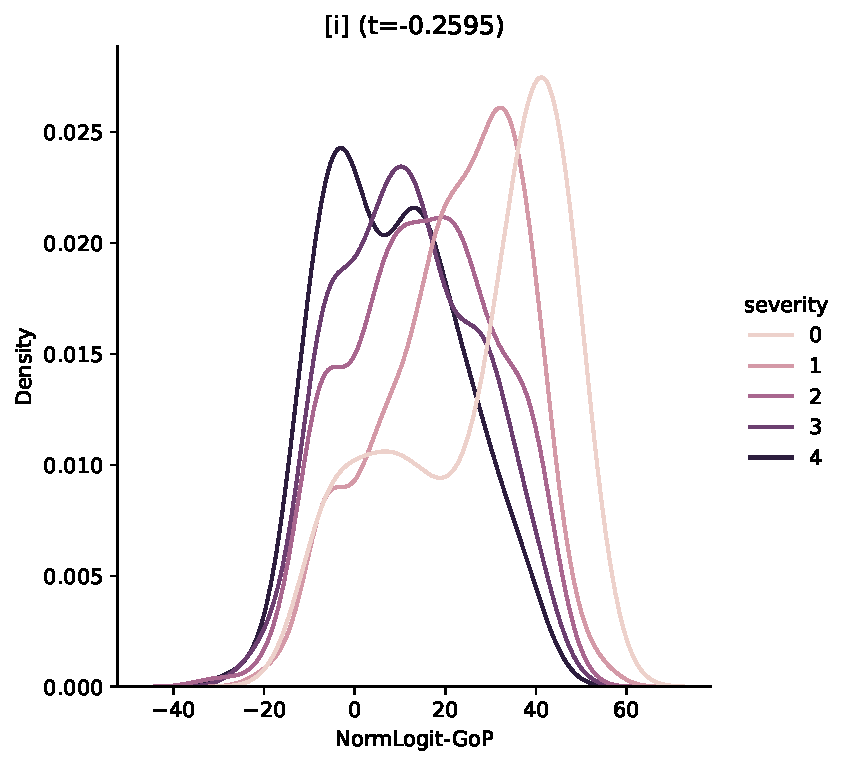
\includegraphics[width=0.43\columnwidth]{figures/korean_i.pdf}}
\subfloat[Korean phoneme \textipa{/m/}.]{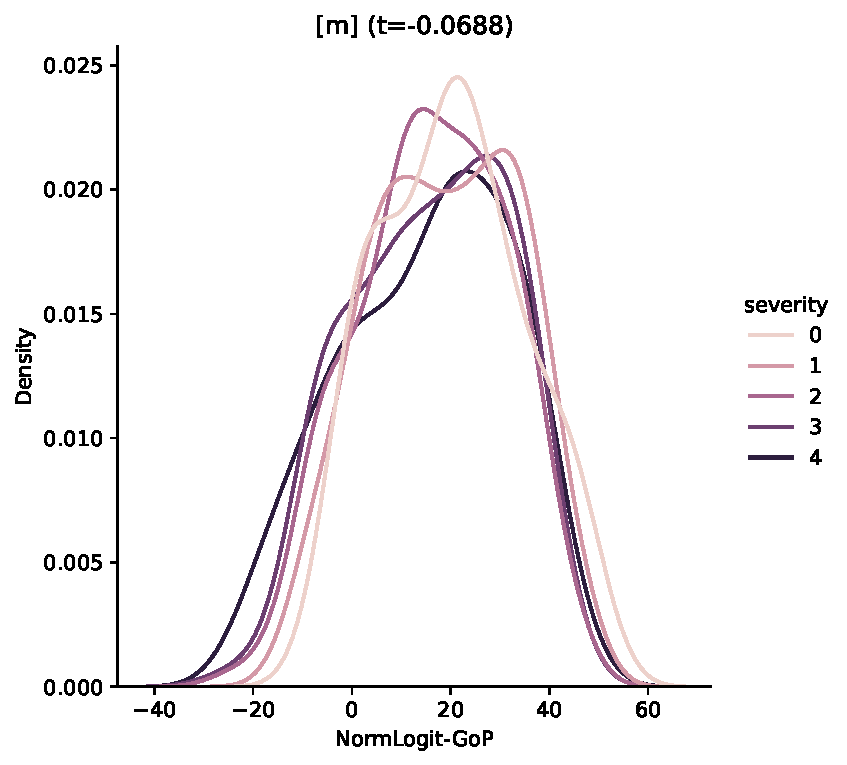
\includegraphics[width=0.43\columnwidth]{figures/korean_m.pdf}}
\vspace{1em}
\caption{
Kendall's $\tau$ distributions for two phonemes by severity.
0:healthy, 1:mild, 2:mild-to-mod., 3:mod.-to-sev., 4:severe.
}
\vspace{-1em}
\label{figs:phones}
\end{figure}

% As certain phonemes have a more significant impact on speech intelligibility than others, 
Identifying which phoneme pronunciation scores highly correlate to speech intelligibility can be useful in the clinical scenario, such as diagnosis and treatment.
For example, as demonstrated in \Cref{figs:samplewise_phones}, one can pinpoint the mispronounced phonemes within a single utterance.


Further, we conduct a quantitative analysis on which phoneme scores highly correlate to speech intelligibility by languages.
Kendall's $\tau$ is calculated for each phoneme between our best-performing Prior+MaxLogit GoP score and the intelligibility scores.
The top-5 phonemes based on correlation are as follows- English: \textipa{/a\textsci/},\textipa{/\textesh/},\textipa{/a\textupsilon/},\textipa{/z/},\textipa{/\textdyoghlig/}; Korean:\textipa{/i/},\textipa{/s/},\textipa{/n/},\textipa{/a/},\textipa{/\textturnv/}; Tamil:\textipa{/\textrtails/},\textipa{/h/},\textipa{/\textteshlig/},\textipa{/z/},\textipa{/a\textsci/}.
In summary, fricative sounds (\textipa{/s/},\textipa{/\textrtails/},\textipa{/\textesh/},\textipa{/z/}) strongly correlates to speech intelligibility across languages, consistent with the previous results \cite{hernandez2019acoustic}.
Affricates (\textipa{/\textteshlig/},\textipa{/\textdyoghlig/}) and diphthongs (\textipa{/a\textsci/},\textipa{/a\textupsilon/}) were shared as the top-5 phoneme list for English and Tamil.
This can be explained by the complexity in the articulation of affricates and diphthongs leading to difficulties in correct pronunciation for speakers with lower speech intelligibility.
On the other hand, Korean showed higher correlations for nasal (\textipa{/n/}) and monophthongs (\textipa{/a/},\textipa{/i/},\textipa{/\textturnv/}).
This may be again related to the movement of the articulators, such as the tongue, velum, and jaw.
We additionally provide the correlation scores of all the phonemes in our repository.\footref{footnote:repo_url}

% \input{sections/5_discussion}
\section{Conclusion} \label{sec:conclusion}
This paper proposes an improved GoP for dysarthria speech intelligibility assessment by using UQ methods.
Expected to alleviate the problem of modern NN's overconfidence, especially for disordered speech, tested UQ methods include (1) normalization of phoneme prediction and (2) modification of the scoring function. 
The experiments were carried out on dysarthric speech datasets in English, Korean, and Tamil.
According to the experimental results, the prior normalized MaxLogit GoP shows the best performance, outperforming both the traditional GoPs and other proposed GoP variants.
Furthermore, to verify the usefulness of our proposed method, an analysis of which phoneme pronunciation scores highly correlate to speech intelligibility is conducted.


\section{Acknowledgements}
This work was supported by Institute of Information \& communications Technology Planning \& Evaluation (IITP) grant funded by the Korea government (MSIT) (No.2022-0-00223, Development of digital therapeutics to improve communication ability of autism spectrum disorder patients).

% A limitation of this study is the requirement for time alignment, which will be addressed in future research. 
% Additionally, other speech dimensions such as prosody must also be taken into consideration for effective speech intelligibility assessment.
% This paper contributes in that it introduces an improved GoP, considering the 


% This paper contributes in that it showcases the effectiveness of GoP, which has previously been underutilized in the study of disordered speech.
% Its ability to provide interpretable results at the phoneme level without the parallel corpus could prove valuable in the clinical field.
% % Secondly, the effectiveness of UQ methods on overconfident predictions from neural networks has been investigated.
% % Experiments verified that UQ methods can address the problem, especially in the disordered speech domain.
% % This research contributes to automatic speech intelligibility assessment by demonstrating the potential use of bot
% % The findings suggest that significant acoustic differences must be taken into account when using probabilities from neural networks, especially in applications to disordered speech.
% A limitation of this study is the requirement for time alignment, which will be addressed in future research. 
% Additionally, other speech dimensions such as prosody must also be taken into consideration for effective speech intelligibility assessment.




% The analysis also reveals that while different phonemes have varying relationships with speech intelligibility across different languages, fricatives tend to have a higher correlation with speech intelligibility.
% The experiments conducted on English, Korean, and Tamil dysarthric speech datasets, results indicate that the prior normalized MaxLogit GoP variant is the most effective. 
% This paper contributes to the field of automatic speech intelligibility assessment, by showcasing the application of improved GoP for disordered speech, especially dysarhtric speech.
% Experimental results imply that significant acoustic differences between dysarthric and healthy must be considered, especially when probabilities from the neural networks are employed.

% This paper contributes in showcasing the effectiveness of UQ methods to alleviate the significant differences between dysarthric and healthy speech.

% The study takes into account the significant differences between dysarthric speech and healthy speech.

% This paper contributes in showcasing the effectiveness of GoP, which has previously been underutilized in the study of disordered speech.
% Its ability to provide interpretable results at the phoneme level without the parallel corpus could prove valuable in the clinical field.
% Moreover, the effectiveness of UQ methods on uncalibrated results from the neural networks has been investigated.
% Experiments verified that UQ methods can address the over-confident and uncalibrated outputs produced by neural networks in the speech domain.

%Limitation

% This paper makes two contributions to the field of automatic speech intelligibility assessment. 
% Firstly, it showcases the effectiveness of GoP, which has previously been underutilized in the study of disordered speech.
% Its ability to provide interpretable results at the phoneme level without the parallel corpus could prove valuable in the clinical field.
% Secondly, the effectiveness of UQ methods on uncalibrated results from the neural networks has been investigated.
% Experiments verified that UQ methods can address the over-confident and uncalibrated outputs produced by neural networks in the speech domain.
% Limitation


% This paper investigates the use of UQ methods to enhance the accuracy of GoP variants for assessing dysarthric speech intelligibility. 
% The study takes into account the significant differences between dysarthric speech and healthy speech.
% Applied UQ methods include (1) scoring function modification and (2) phoneme prediction modification.
% Tested on TORGO English, QoLT Korean, and SSNCE Tamil dysarthric speech datasets, the best GoP variant is found to be prior normalized MaxLogit GoP.
% Further analysis of each phoneme implies while phonemes have different relations to speech intellgiblity by languages, fricative \textipa{/s/} shared the pattern to have high correlations to speech intelligibility.

% While the overall results of the experiments using UQ methods outperformed the baseline experiments, Normalized MelLogit-Gop showed the greatest correlation with the intelligibility scores.
% Experimental results suggest that traditional GoPs were not properly calibrated, and UQ methods can effectively address this issue.
% Furthermore, we conduct phoneme-level analysis to find frequently mispronounced phonemes by each language.
% This paper makes two contributions to the field of automatic speech intelligibility assessment. 
% Firstly, it showcases the effectiveness of GoP, which has previously been underutilized in the study of disordered speech.
% Its ability to provide interpretable results at the phoneme level without the parallel corpus could prove valuable in the clinical field.
% Secondly, the effectiveness of UQ methods on uncalibrated results from the neural networks has been investigated.
% Experiments verified that UQ methods can address the over-confident and uncalibrated outputs produced by neural networks in the speech domain.
%Limitation

% an improved version UQ method on GoP, and demonstrates its effectiveness 

% A limitation of our study lies in the discrepancy between the evaluation and labeling methods.
% While the labels were assigned based on a speaker level, we assessed the intelligibility scores on an utterance level, assuming that all utterances from the speaker had the same level of intelligibility.
% To alleviate such issues, we plan to aggregate the intelligibility scores of individual utterances into speaker-level scores.
% Another limitation is that we did not provide information on how each phoneme was mispronounced. 
% Hence, we plan to develop a model that can provide this level of detail in our future work.


%% Consider Percpetual evaluation + other aspects other than pronunciation.

% , which will help us better understand the specific areas where non-native speakers struggle with pronunciation.
% no need of large trained models





% First, the analysis is limited to sentences. 
% Future work includes 



% In addition, cross-lingual representations from the wav2vec2 XLS-R model are extracted, to overcome the limitations of most GoPs where language-specific acoustic models with large amounts of training data is required.

% The GoP with UQ method is tested on dysarthric datasets in English, Korean, and Tamil, and results in higher Kendall's rank coefficients with speech intelligibility classes than previous experiments using GMM-GoP, NN-GoP, ASR free-GoP, and SSL-GoP.






\bibliographystyle{IEEEtran}
\bibliography{mybib}

\end{document}
